\documentclass[MASTER.tex]{subfiles} 
\begin{document} 
	
	
	\begin{frame}
		\huge
		\[ \mbox{Machine Learning with Python} \]
	\end{frame}
	
	%===========================================================%%=======================================================================%
\begin{frame}
\Large
\textbf{What is Machine Learning}
\begin{itemize}
\item Machine Learning is a discipline involving algorithms designed to find patterns in and make predictions about data. 
\item It is nearly ubiquitous in our world today, and used in everything from web searches to financial forecasts to studies of the nature of the Universe. 
%This tutorial will offer an introduction to scikit-learn, a python machine learning package, and to the central concepts of Machine Learning.
\end{itemize}
 

\end{frame}

%========================================================================%

\begin{frame}
\Large
\textbf{What is Machine Learning}
\begin{itemize}
	\item	
Machine learning is a type of artificial intelligence (AI) that provides computers with the ability to learn without being explicitly programmed. 
\item Machine learning focuses on the development of computer programs that can teach themselves to grow and change when exposed to new data. 
\end{itemize}
\end{frame}
%========================================================================%

\begin{frame}
\Large
\textbf{What is Machine Learning}
\begin{itemize}
	\item The process of machine learning is similar to that of data mining. Both systems search through data to look for patterns. 
	\item However, instead of extracting data for human comprehension -- as is the case in data mining applications -- machine learning uses that data to improve the program's own understanding. \item Machine learning programs detect patterns in data and adjust program actions accordingly. 
\end{itemize}
\end{frame}
%=======================================================================%
%\begin{frame}
%\Large	\textbf{MachineLearning}\\
%	We will introduce the basic categories of learning problems and how to implement them using scikit-learn. From this foundation, we will explore practical examples of machine learning using real-world data, from handwriting analysis to automated classification of astronomical images.
%
%\end{frame}
%========================================================================%
\begin{frame}
	\begin{figure}
\textbf{	Recommender Engines}
\centering
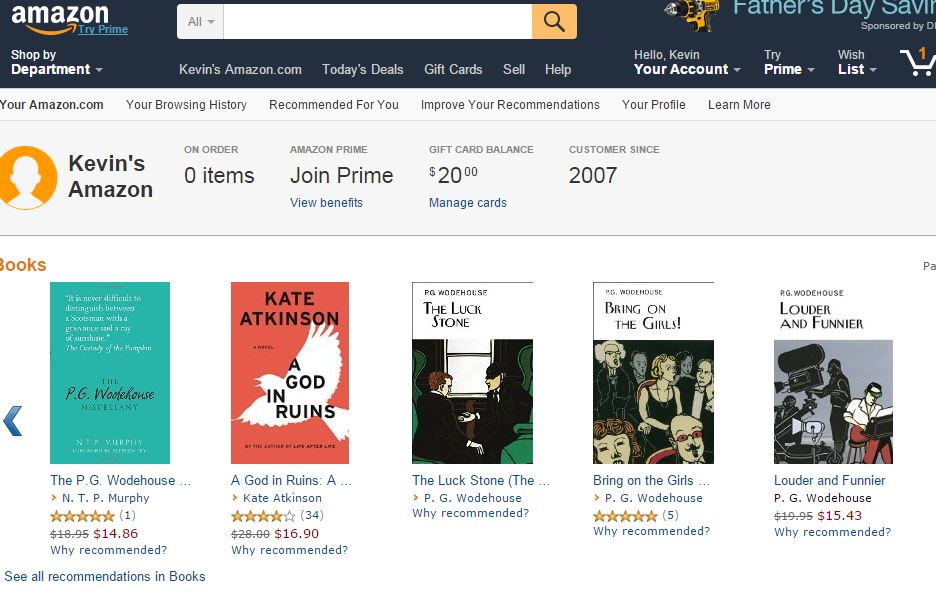
\includegraphics[width=1.1\linewidth]{amazonrecommends}

\end{figure}

	
\end{frame}	
%========================================================================%

\begin{frame}
	\LARGE
	\textbf{Facebook's Newsfeed}
	\begin{itemize}
	\item For example, Facebook's News Feed changes according to the user's personal interactions with other users. 
	\item If a user frequently tags a friend in photos, writes on his wall or "likes" his links, the News Feed will show more of that friend's activity in the user's News Feed due to presumed closeness.
	\end{itemize}
	
	
\end{frame}
\end{document}